\section{Modelo de Incentivos para Desarrolladores}
\noindent
El \pidc, (\textit{Developer Incentive Protocol}, o DIP), incluye dos procesos: la valuación de las {\dapp}s y la distribución de los incentivos.

Por un lado, la construcción de un sistema de valuación robusto puede brindarle a los desarrolladores una plataforma conveniente y efectiva para promover aplicaciones y brindarles a sus usuarios un sistema de recomendaciones fiable; tal como sucede en la plataforma App Store, las buenas aplicaciones se nmuestran primero en los listados y, debido a ello, reciben más atención de los usuarios. Por otro lado, los usuarios reciben una mejor experiencia cuando encuentran aplicaciones de alta calidad directamente en ese listado. Más aun, la valuación de las aplicaciones puede ser utilizada en la búsqueda por palabras clave.

Tal como ocurre en los motores de búsqueda, y en las plataformas de \textit{e-commerce}, el listado de aplicaciones ordenado por palabras clave y de acuerdo a su valuación en los resultados de la búsqueda contribuye a la satisfacción de los usuarios.

Como vimos en la sección \ref{sec:antecedentes}, el propósito del \pidc es el de brindar incentivos a todos los desarrolladores de aplicaciones de calidad, aumentando así los incentivos de esos desarrolladores para diseñar buenas {\dapp}s y promoviendo, en paralelo, el desarrollo del ecosistema.

De esto se desprende que el segundo proceso en el modelado del \pidc es el diseño de un mecanismo equitativo de incentivos, en concordancia con la valuación de cada \dapp.

\subsection{Representación del modelo}
\label{subsection:parameters}
\noindent
En esta sección presentamos la notación y símbolos necesarios en el modelo DIP.

\begin{itemize}
	\item $\mathcal{A}=\{a_1,a_2,\ldots,a_m\}$ representa el conjunto de usuarios que participan en el sistema de valuación durante un periodo dado. Utilizamos votantes para denotar a esos usuarios. Nótese que un usuario está definido como votante únicamente si realiza una llamada a algunas {\dapp}s EOA (Cuenta de Propiedad Externa, o \textit{External Owned Account} en inglés) dentro de un periodo dado. Defínase
	  $$\mathcal{A}^*=\{a_1,a_2,\ldots,a_m,a_{m+1},\ldots,a_{m^*}\}$$
	como el conjunto de todos los usuarios en la comunidad durante el mismo periodo de tiempo; esto es, $m^*-m$ usuarios que no invocan ninguna \dapp.
  \item $\mathcal{D}=\{d_1,\ldots,d_n\}$ representa el conjunto de {\dapp}s durante un periodo de tiempo dado.
  \item $e_{ij},i=1,2,\ldots,m, j=1,2,\ldots,n$ representa la cantidad de veces que el votante $a_i$ invoca la \dapp $d_j$. Debido al carácter público y descentralizado del blockchain, el modelo DIP difiere del de otros sistemas de valuación en mercados de aplicaciones centralizadas. Generalmente hablando, DIP valúa las {\dapp}s de acuerdo al comportamiento de las invocaciones realizadas por los usuarios en un entorno descentralizado. Los detalles del análisis se brindan en la siguiente sección de este documento.

  \item $\nr_i, i=1,2,\ldots,m$ representa la capacidad de voto de un votante $a_i$ durante un periodo de tiempo dado.
  \cite{Nebulasyellowpaper} demuestra que el valor NR de un usuario es una medida efectiva del valor de su cuenta. Así, en DIP, NR se utiliza también como un criterio significativo para decidir la capacidad de voto de los votantes.
  \item $\nr_{ij}, i=1,2,\ldots,m,j=1,2,\ldots,n$ representa el valor contributivo de un votante $a_i$ a una \dapp $d_j$, que puede considerarse como el número de votos que $a_i$ está dispuesto a otorgar a $d_j$.

  \item $S_j, j=1,2,\ldots,n$ representa el puntaje de la valuación de una \dapp $d_j$, que está determinado por el valor recibido por parte de todos sus votantes. Intuitivamente, el puntaje de valuación determina la posición de las {\dapp}s en la lista de valuación.

  	\item $M$ representa el total del fondo de incentivos para desarrolladores, que tiene su origen en las recompensas por nuevos bloques. La recompensa real se reducirá adecuadamente de acuerdo con la tasa de participación de toda la comunidad durante el período de tiempo dado.
   \item $U_j, j=1,2,\ldots,n$ representa el incentivo final de la \dapp $d_j$, que se determina por el total disponible en el fondo de incentivos, y por el puntaje de valuación de las {\dapp}s.
 \end{itemize}
   \begin{figure}
   	\centering
   	%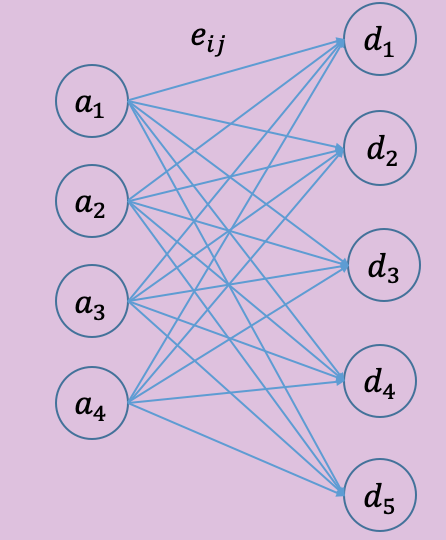
\includegraphics[width = 0.4\textwidth]{../common/m2.png}
   	\begin{tikzpicture}
\pgfmathsetmacro{\XTD}{3.8}
\pgfmathsetmacro{\YTD}{1.2}

\tikzset{
  node/.style={draw, circle, on grid, align=center, minimum height=2ex},
}

\node[node] (d1) at (\XTD, 2*\YTD) {$d_1$};
\node[node] (d2) at (\XTD, \YTD) {$d_2$};
\node[node] (d3) at (\XTD, 0) {$d_3$};
\node[node] (d4) at (\XTD, -1*\YTD) {$d_4$};
\node[node] (d5) at (\XTD, -2*\YTD) {$d_5$};

\node [right=0.05 of d1] {${S}_{1}$};
\node [right=0.05 of d2] {${S}_{2}$};
\node [right=0.05 of d3] {${S}_{3}$};
\node [right=0.05 of d4] {${S}_{4}$};
\node [right=0.05 of d5] {${S}_{5}$};

\node[node] (a1) at (-\XTD, 1.5*\YTD) {$a_1$};
\node[node] (a2) at (-\XTD, 0.5*\YTD) {$a_2$};
\node[node] (a3) at (-\XTD, -0.5*\YTD) {$a_3$};
\node[node] (a4) at (-\XTD, -1.5*\YTD) {$a_4$};

\node [left=0.05 of a1] {${\nr}_{1}$};
\node [left=0.05 of a2] {${\nr}_{2}$};
\node [left=0.05 of a3] {${\nr}_{3}$};
\node [left=0.05 of a4] {${\nr}_{4}$};

\draw[->, >=stealth'] (a1) to (d1);
\draw[->, >=stealth'] (a1) to (d2);
\draw[->, >=stealth'] (a1) to (d3);
\draw[->, >=stealth'] (a1) to (d4);
\draw[->, >=stealth'] (a1) to (d5);

\draw[->, >=stealth'] (a2) to (d1);
\draw[->, >=stealth'] (a2) to (d2);
\draw[->, >=stealth'] (a2) to (d3);
\draw[->, >=stealth'] (a2) to (d4);
\draw[->, >=stealth'] (a2) to (d5);

\draw[->, >=stealth'] (a3) to (d1);
\draw[->, >=stealth'] (a3) to (d2);
\draw[->, >=stealth'] (a3) to (d3);
\draw[->, >=stealth'] (a3) to (d4);
\draw[->, >=stealth'] (a3) to (d5);

\draw[->, >=stealth'] (a4) to (d1);
\draw[->, >=stealth'] (a4) to (d2);
\draw[->, >=stealth'] (a4) to (d3);
\draw[->, >=stealth'] (a4) to (d4);
\draw[->, >=stealth'] (a4) to (d5);

\node at (0, 2*\YTD) {$e_{ij}$};

\end{tikzpicture}

   	\caption{Interacciones entre votantes y {\dapp}s \label{fig:interact}}
   \end{figure}
  Para sumarizar, las interacciones entre votantes y {\dapp}s se puede representar mediante un gráfico bipartito en la figura \ref{fig:interact}.

 \subsection{Acción de voto}
 \label{subsection:voting}
 \noindent
  En cualquier App Store centralizada\footnote{\url{https://en.wikipedia.org/wiki/App\_store}}, el sistema puede almacenar información específica tal como la cantidad de veces que una App fue descargada, lo cual es un factor clave para determinar su valuación. No obstante, en el mundo del blockchain, la forma en la que los usuarios utilizan las {\dapp}s es mediante la invocación de las direcciones de contratos inteligentes; esto se puede cuantificar mediante la cantidad de veces que un usuario $a_i$ invoca la \dapp $d_i$, algo denotado por $e_{ij}$. Comparado a la información tradicional acerca de cantidad de descargas, la metodología que usa DIP, de tomar la información de las llamadas a {\dapp}s como parámetro de valuación, tiene las siguientes ventajas:

 \begin{itemize}
 	\item El número de llamadas se almacena en el blockchain, que es muy resistente al fraude, es más abierto y transparente, en comparación con otros métodos centralizados tales como el registro del número de descargas.
 	\item El número de llamadas es un parámetro más detallado que la cantidad de descargas, ya que el número de descargas sólo registra el comportamiento de un usuario por única vez, mientras que el registro de cantidad de llamadas a una \dapp señala, además, la fidelidad de ese usuario con la aplicación. En consecuencia, el número de llamadas es un parámetro más razonable para reflejar el comportamiento real de los usuarios.

\end{itemize}

 En realidad existe más información disponible cuando los usuarios invocan una llamada a las {\dapp}s. Por ejemplo, la cantidad de \textit{gas} que se ha utilizado, y las transferencias de tokens involucradas en una transacción. Sin embargo, DIP no toma estos datos en consideración por dos motivos.

 Primero, la cantidad de \textit{gas} consumido depende de la cantidad de instrucciones ejecutadas en el contrato inteligente cada vez que un usuario invoca una \dapp, algo que no guarda relación con la calidad intrínseca de la \dapp en cuestión. Más aun, en el sistema actual de Nebulas, la cantidad promedio de \textit{gas} consumido durante cada invocación está en el orden de $10^{-8}$ NAS, algo insignificante.

 Segundo, la razón por la que no se toman en cuenta las transferencias de tokens es la falta de un método efectivo contra la manipulación. Intuitivamente sabemos que la voluntad de los usuarios de pagar tokens adicionales cada vez que llaman a una \dapp es algo que mejora la valuación de esta. Sin embargo, en la práctica, cuando un usuario decide pagar tokens para utilizar una \dapp, el destino final de esos tokens puede ser cualquiera de estos tres casos:

  \begin{enumerate}
  	 \item Los tokens quedan finalmente en posesión del desarrollador de la \dapp. En este caso, es probable que el usuario pague voluntariamente por el uso de la \dapp. Como su desarrollador recibe beneficios por parte del usuario, no es relevante incrementar aun más la valuación de su \dapp.
  	\item La misma naturaleza de la \dapp requiere una transferencia de tokens —por ejemplo {\dapp}s de apuestas— lo que lleva a una gran cantidad de tokens transferidos entre el usuario y la \dapp, algo que es normal y aceptable. Sin embargo, la valuación de estas {\dapp}s no se debería incrementar por ello, debido al hecho de que el propósito de esas transferencias es la de obtener ganancias, algo que no refleja la calidad de la \dapp.
   \item El desarrollador de la \dapp afirma que todos los tokens recibidos por la \dapp serán devueltos al usuario. Esto constituye en sí mismo un acto de manipulación, que se agravaría si la \dapp recibe recompensas y valuación por ello.
  \end{enumerate}
  En la práctica, sin analizar el código fuente de los contratos inteligentes, no es posible determinar en cuál de estos casos cae cada transferencia de tokens entre usuarios y  {\dapp}s y en todo caso en ninguno de ellos se amerita otorgar incentivos, de modo que el algoritmo del DIP no tomará en cuenta la transferencia de tokens.

  En el modelo DIP, un usuario $a_i \in \mathcal{A}$ se ve esencialmente como una dirección Nebulas. Tal como se refiere en \cite{Nebulasyellowpaper}, un único usuario puede controlar múltiples direcciones. Debido a que no hay costo alguno en la creación de una dirección Nebulas, el usuario podría crear numerosas direcciones con el fin de votar, algo que se conoce como el ataque Sybil. Similarmente, un desarrollador podría dividir sus \dapp en distintas direcciones —esto es, dividir su \dapp en distintas {\dapp}s de baja calidad, y obtener recompensas por todas las {\dapp}s asociadas a esas direcciones. Mientras tanto, un desarrollador podría pagarle a uno o más usuarios para votar por su \dapp.

  Hemos analizado todas las manipulaciones descriptas más arriba al momento de diseñar DIP, y les hemos dado solución. Los detalles de los mecanismos antifraude de DIP se encuentran en la sección \ref{section:properties}.

  \subsection{Intervalo de muestreo}
  \label{subsection:interval}
  \noindent
  En la sección \ref{subsection:parameters}, hemos mostrado que NR es un criterio significativo para determinar la capacidad de voto de cada usuario. Sin perjuicio de ello y de acuerdo a la definición en \cite{Nebulasyellowpaper}, el periodo de muestreo de los datos para el DIP es mucho mayor que el necesario para NR, lo que implica que durante el proceso de registro del comportamiento de las invocaciones de los usuarios, el valor NR podría fluctuar, incluso significativamente.

  Un enfoque simplista es sincronizar el período de muestreo de los datos NR y los datos DIP. En la práctica, sin embargo, se ha visto que la utilización de periodos cortos de tiempo (un día, por ejemplo), son insuficientes para la mayoría de los usuarios, ya que muchos de ellos realizan invocaciones en periodos de tiempo mayores, de modo que tiene poco sentido valuar las {\dapp}s de este modo cuando el comportamiento de los usuarios es disperso, y no hay garantía de que se satisfagan las condiciones enumeradas en la sección \ref{section:properties}.

  De este modo, nuestra estrategia es la de extender apropiadamente el periodo de muestreo para recoger suficiente información sobre el comportamiento de las invocaciones, y encuadrar la variación del valor NR de los usuarios de forma simultánea. La variación del valor NR de una dirección se muestra en la figura \ref{fig:nr}. Allí dividimos el proceso completo de DIP en distintos periodos de tiempo. De acuerdo a los datos acerca de las variaciones de NR, se elige un entero $t$ tal que la variación de NR dentro de $t$ días menos que el umbral $\tau$ es apto para la mayoría de los usuarios. Tomamos $t$ días como un periodo de muestreo, reuniendo el promedio de valores NR de los votantes y los datos de invocación durante ese periodo para computar el puntaje de valuación de las {\dapp}s y las recompensas finales para sus desarrolladores. Luego tomamos los datos medios de todos los períodos de tiempo durante el proceso de valuación como resultados finales.

  \begin{figure}
  	\centering
  	\pgfplotstableread[col sep=comma]{../common/gateionr.csv}\datatable

\begin{tikzpicture}
  \begin{axis}[
%ticks=none,
ylabel={NR value},
xlabel={date},
%xtick={0,10,20,30,40,50,60},
%xlabel={时间(天)}
legend style={fill=none},
xtick={0, 56},
xticklabels={2018/07/31, 2018/09/25},
extra x ticks={1, 2, ..., 55},
      extra x tick style={
        xticklabels={,,},
      },
%xticklabels from table={\datatable}{record},
width=.75\textwidth,
    ]
\addplot [mark=., color=blue] table [x expr=\coordindex, y=nr, col sep=comma] {../common/gateionr.csv};

\draw[dashed, color=gray] (axis cs:0, 340000000) -- ( axis cs:0,
450000000) ;
\draw[dashed, color=gray] (axis cs:6, 340000000) -- ( axis cs:6,
450000000) ;
\draw[dashed, color=gray] (axis cs:21, 340000000) -- ( axis cs:21,
450000000) ;
\draw[dashed, color=gray] (axis cs:35, 340000000) -- ( axis cs:35,
450000000) ;
\draw[dashed, color=gray] (axis cs:56, 340000000) -- ( axis cs:56,
450000000) ;

\draw[<->, color=gray] (axis cs:0, 445000000) -- node[ color=black, fill=violet!25, anchor=center] {\small $t_1$} (axis cs:6, 445000000);
\draw[<->, color=gray] (axis cs:6, 445000000) -- node[ color=black, fill=violet!25,
anchor=center] {\small $t_2$} (axis cs:21, 445000000);
\draw[<->, color=gray] (axis cs:21, 445000000) -- node[ color=black, fill=violet!25,
anchor=center] {\small $t_3$} (axis cs:35, 445000000);
\draw[<->, color=gray] (axis cs:35, 445000000) -- node[ color=black, fill=violet!25,
anchor=center] {\small $t_4$} (axis cs:56, 445000000);
\end{axis}

\end{tikzpicture}


  	\caption{\label{fig:nr} Gráfico de la variación de NR de una dirección en la red Nebulas. La dirección mainnet es \texttt{n1Ugq21nif8BQ8uw81SwXHK6DHqeTEmPRhj}.}
  \end{figure}